\section{Reduced-Physics Model}

This section describes the derivation of the RPM model for the ablating TPS surface. The model is composed of two components: (1) a thermal solver to capture the one-dimensional distribution of temperature across the ablating material, and (2) an elasticity solver to capture the one-dimensional mesh motion as a function of the surface temperature. The interface between the thermal solver and the moving mesh is achieved using a B' table, which determines the surface recession velocity as a function of the wall temperature.

\subsection{Computational Domain}

Consider a $2$ mm Titanium slab as shown in Fig.~\ref{fig_ablation_domain}. The geometry, material properties, and boundary conditions are summarized in Table~\hl{x}. The left surface is exposed to the hypersonic flow (Neumann boundary condition), while the right surface is perfectly insulated (adiabatic boundary condition). 

\begin{figure}[h]
    \centering
    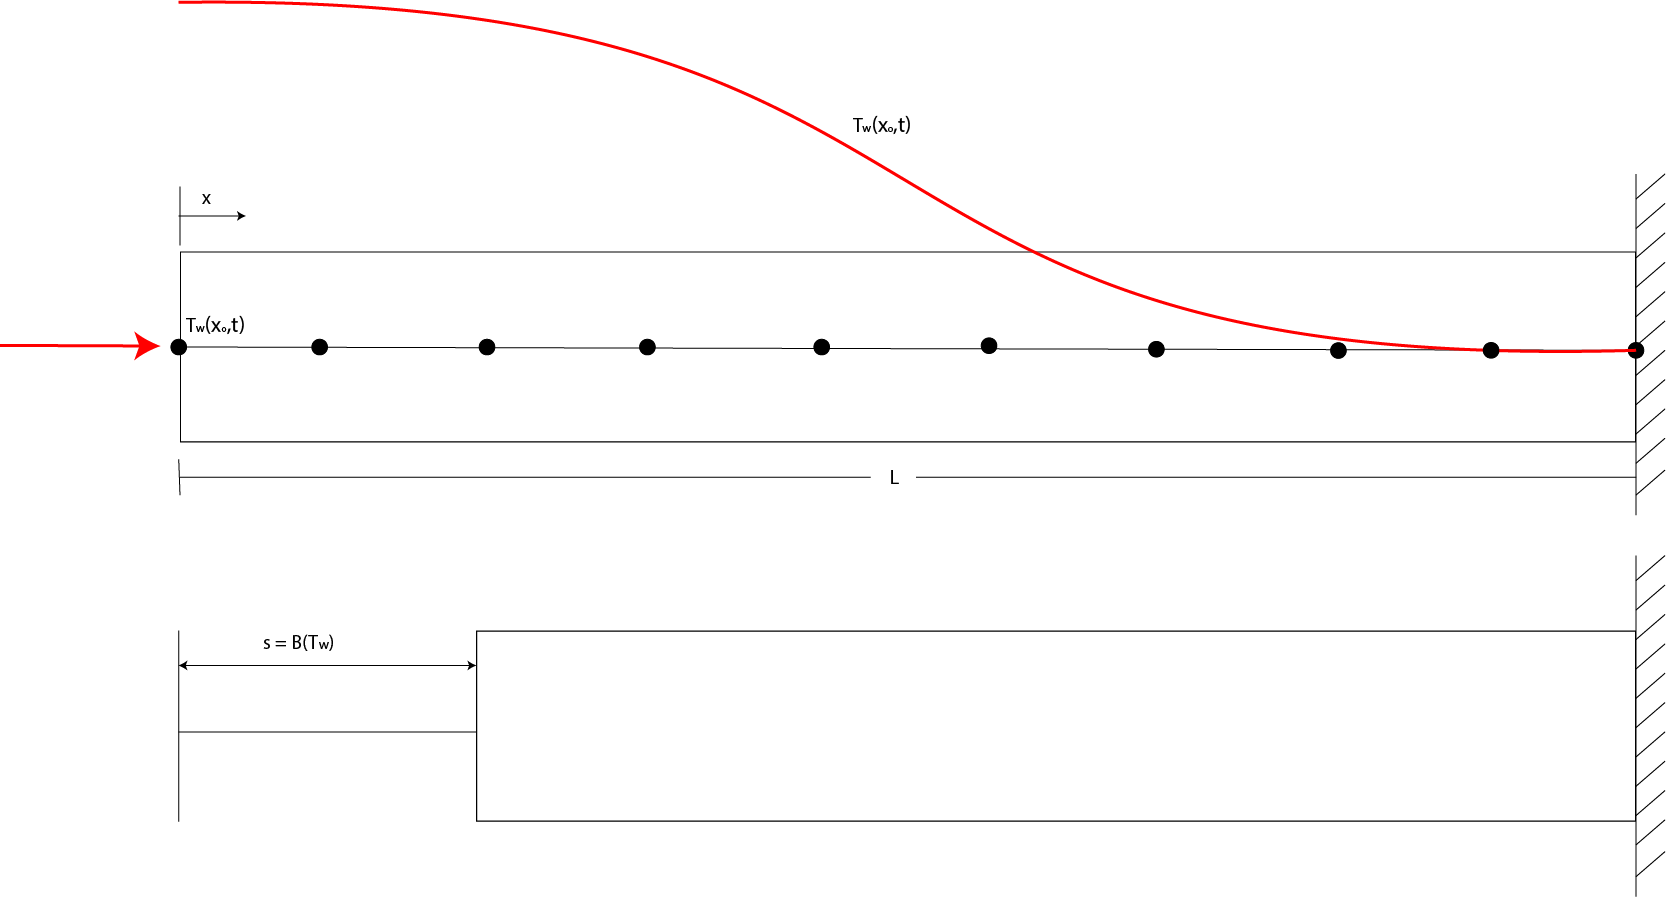
\includegraphics[width=0.9\textwidth]{./figs/ablation.png}
    \label{fig_ablation_domain}
\end{figure}

\begin{table}[h]
    \begin{tabular}{cccc}
        Material & Density, $[\text{kg}/\text{m}^3]$ & Thermal Conductivity, $\text{W}/{\text{m}\text{K}}$ & Specific Heat, $[\text{J}/\text{kg}\text{K}]$\\
        \hline
        \hline
        Tungstenn & x & x & x\\
        \hline
        \hline
    \end{tabular}
\end{table}

\subsection{Governing Equations}

The governing equations for a non-decomposing ablator involves the energy equation with a temperature advection term to account for the moving boundary. An Arbitrary Lagrangian-Eulerian description (ALE) is adopted to incorporate the effects of mesh motion into the energy equation. The ALE approach assumes the computational mesh moves with a velocity $\mathbf{v}(x,t)$ that is different to the material velocity $\mathbf{w}(x,t)$. These effects are taken into 

moves the mesh independently of the material movement, 

\begin{subequations}\label{eqn_pde}
    \begin{align}
        \rho c_p\ppt{T} + \rho c_p\left(\mathbf{w}(x,t) - \mathbf{v}(x,t)\right)\cdot\nabla T - \nabla\cdot (\mathbf{k} \nabla T) &= 0,\ x\in\Omega \\
        \nabla\cdot\boldsymbol{\sigma}(\mathbf{u}) &= 0\\
        -\mathbf{k}\nabla T\cdot \vn  &= q_b(x,t),\ x\in\Gamma_q \\
        T(x,0) &= T_0(x),\ x\in\Omega
    \end{align}
\end{subequations}

-------------------------------

The following simplifications are introduced in the FOM \hl{x} to aid in the derivation of the RPM,
\begin{enumerate}
    \item The material properties are independent of temperature.
    \item The domain is one dimensional.
    \item The spatial discretization is coarse-grained.
    \item ...
\end{enumerate}
With these 


With the inclusion of the physical assumptions, the FOM in \hl{x} reduces to the following one-dimensional energy equation with the temperature advection term for the moving mesh,
\begin{subequations}
    \begin{align}
        \rho c_p\left(\frac{\partial T}{\partial t} - v(x,t)\frac{\partial T}{\partial x}\right) - \frac{\partial}{\partial x}\left(k\frac{\partial T}{\partial x}\right) &= 0\\
        \frac{\partial}{\partial x}\left(E\frac{\partial u}{\partial x}\right) &= 0\label{eqn_elasticity_1d}\\
        k\frac{\partial T}{\partial x}\Bigg|_{x=0} &= q(t)\label{eqn_neumann_bc}\\
        k\frac{\partial T}{\partial x}\Bigg|_{x=\ell} &= 0\\
        u(0,t) &= v(t) * (t - t_0)\\
        u(\ell,t) &= 0
    \end{align}
\end{subequations}

\subsection{Numerical Solution}

A numerical solution based on the FEM method is adopted for the governing PDEs. 

\subsubsection{Elasticity Solver}

Assuming the Young's modulus is constant, the PDE simplifies to,
\begin{equation}
    \frac{\partial^2 u}{\partial x^2} = 0
\end{equation}
which has the analytical solution,
\begin{equation}
    u(x,t) = a(t)x + b(t)
\end{equation}
Using the boundary conditions leads to,
\begin{equation}
    u(x,t) = u(0,t) * \left(1 - \frac{x}{\ell}\right)
\end{equation}
The mesh velocity is the time derivative of the displacement,
\begin{equation}
    v(x,t) = \frac{\partial u(x,t)}{\partial t} = v(t)\left(1 - \frac{x}{\ell}\right)
\end{equation}

\subsubsection{Thermal Solver}

Let $\phi^{(e)}_i(x)$ with $i=1,2$ be two linear shape defined over the element $e_i=[x_{i},x_{i+1}]$ with length $h_e=x_{i+1} - x_i$,
\begin{equation}
    \phi^{(e)}_1(x) = \left\{\begin{matrix}
        \frac{x_{i+1} - x}{h_e},\quad x\in[x_i,x_{i+1}]\\
        0, \quad \text{otherwise}
    \end{matrix}\right.,\quad\phi^{(e)}_2(x) = \left\{\begin{matrix}
        \frac{x - x_i}{h_e},\quad x\in[x_i,x_{i+1}]\\
        0, \quad \text{otherwise}
    \end{matrix}\right.
\end{equation}
Letting,
\[
    x(\xi) = \frac{1-\xi}{2}x_i + \frac{1 + \xi}{2}x_{i+1}
\]
for $\xi\in[-1,1]$,
\begin{equation}
    \hat{\phi}_1^{(e)}(\xi) = \frac{1 - \xi}{2},\quad \hat{\phi}_2^{(e)}(\xi) = \frac{1 + \xi}{2}
\end{equation}

Multiply through by the test function,
\begin{equation}
    \int_{\Omega}\left[\rho c_p\frac{\partial T}{\partial t} - \rho c_p v(x,t)\frac{\partial T}{\partial x} - \frac{\partial}{\partial x}\left(k\frac{\partial T}{\partial x}\right)\right]\phi_i(x)dx = 0
\end{equation}
.
.
.
\begin{equation}
    \int_{\Omega}\rho c_p\frac{\partial T}{\partial t}\phi_i(x)dx - \int_{\Omega}\rho c_p v(x,t)\frac{\partial T}{\partial x}\phi_i(x)dx + \int_{\Omega} k\frac{\partial T}{\partial x}\frac{\partial\phi_i(x)}{\partial x} dx = k\frac{\partial T}{\partial x}\phi_i(x)\Bigg|_{\partial\Omega}
\end{equation}
Perform the finite-element approximation,
\begin{equation}
    T(x,t)\approx\sum_jT_j(t)\phi_j(x)
\end{equation}
and define the matrix elements,
\begin{align}
    M_{ij} &= \int_{\Omega}\rho c_p\phi_i(x)\phi_j(x)dx\\
    C_{ij}(t) &= \int_{\Omega}\rho c_p v(x,t) \frac{\partial\phi_j}{\partial x}\phi_i(x)dx\\
    K_{ij} &= \int_{\Omega}k\frac{\partial\phi_i(x)}{\partial x}\frac{\partial\phi_j(x)}{\partial x}dx\\
    f_i(t) &= k\frac{\partial T}{\partial x}\phi_i(x)\Bigg|_{\partial\Omega}
\end{align}
The time-dependent finite-dimensional ODE system for nodal temperatures $\mathbf{T}(t)$, including the ALE-induced advection effect from mesh motion, is given as,
\begin{equation}
    \mathbf{M}\frac{d\mathbf{T}}{dt} + \left(\mathbf{K} - \mathbf{C}(t)\right)\mathbf{T} = \mathbf{f}(t)
\end{equation}

The element-level expressions for the mass, stiffness, advection, and forcing vectors are given as,
\begin{align}
    M^{(e)}_{mn} &= \int_{x_i}^{x_{i+1}}\rho c_p\phi_m(x)\phi_n(x)dx = \rho c_p \frac{h_e}{6}\begin{pmatrix}
        2 & 1 \\ 1 & 2
    \end{pmatrix}\\
    K^{(e)}_{mn} &= \int_{x_i}^{x_{i+1}} k \frac{\partial \phi_m}{\partial x}\frac{\partial \phi_n}{\partial x} dx = \frac{k}{h_e}\begin{pmatrix}
        1 & -1 \\ -1 & 1
    \end{pmatrix}\\
    C^{(e)}_{mn}(t) &= \int_{x_i}^{x_{i+1}}\rho c_p v(x,t) \frac{\partial \phi_n(x)}{\partial x}\phi_m(x) dx\\
    f^{(e)}_1(t) &= \left(q(t),0\right)^T
\end{align}

\subsection{Coarse Graining}

\begin{equation}
    \vA(\vu)\dot{\vu} = \left(\vB(\vu) - \vC(\vu,t)\right)\vu + \vf(t)
\end{equation}
so that,
\begin{equation}
    \dot{\vu} = \vr(\vu,t) = \vA(\vu)^{-1}\left[\left(\vB(u) - \vC(\vu,t)\right)\vu + \vf(t)\right]
\end{equation}
The resolved dynamics,
\begin{align}
    \vr^{(1)}(\vu,t) &= \cP\left[\vPhi^+\vr(\vu,t)\right]\\
    &=\cP\left[\vPhi^+\vA^{-1}(\vu)\vB(\vu)\vu - \vPhi^+\vA^{-1}(\vu)\vC(\vu,t)\vu + \vPhi^+\vA^{-1}(\vu)\vf(t)\right]
\end{align}
\subsection{Numerical Simulation Results}

